\begin{center}
    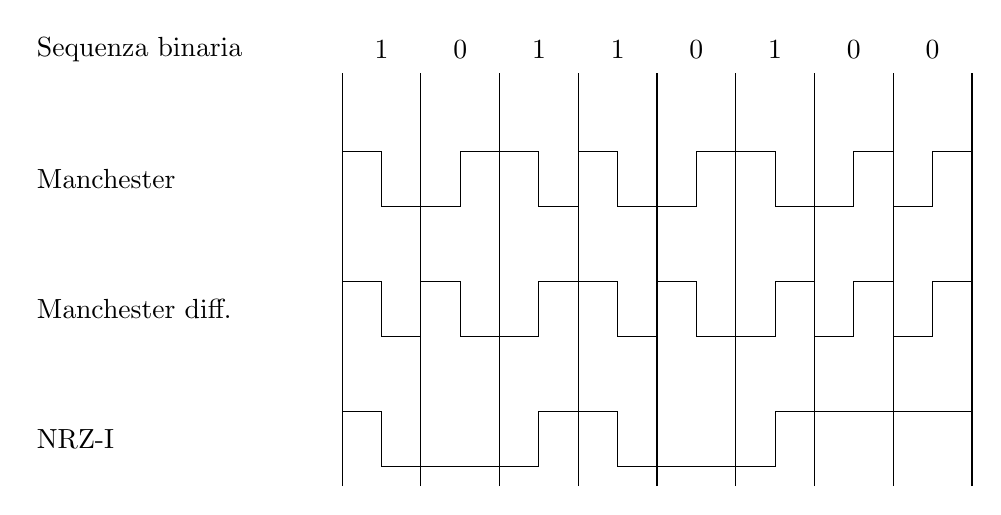
\begin{tikzpicture}
        %%%%%%%%% Barre %%%%%%%%%%
        \foreach \x in {4,...,12}
            \draw (\x,-0.25) -- (\x,5);

        %%%%%%%%% Numeri %%%%%%%%%
        \node at (4.5,5.3) {1};
        \node at (5.5,5.3) {0};
        \node at (6.5,5.3) {1};
        \node at (7.5,5.3) {1};
        \node at (8.5,5.3) {0};
        \node at (9.5,5.3) {1};
        \node at (10.5,5.3) {0};
        \node at (11.5,5.3) {0};

        %%%%%%%%% NRZ-I %%%%%%%%%%
        \draw (4,0.7) -- (4.5,0.7) -- (4.5,0) -- (6.5,0) -- (6.5,0.7) -- (7.5,0.7) -- (7.5,0) -- (9.5,0) -- (9.5,0.7) -- (12,0.7);

        %%%% Manchester Diff. %%%%
        \draw (4,2.35) -- (4.5,2.35) -- (4.5,1.65) -- (5,1.65);
        \draw (5,2.35) -- (5.5,2.35) -- (5.5,1.65) -- (6,1.65);
        \draw (6,1.65) -- (6.5,1.65) -- (6.5,2.35) -- (7,2.35);
        \draw (7,2.35) -- (7.5,2.35) -- (7.5,1.65) -- (8,1.65);
        \draw (8,2.35) -- (8.5,2.35) -- (8.5,1.65) -- (9,1.65);
        \draw (9,1.65) -- (9.5,1.65) -- (9.5,2.35) -- (10,2.35);
        \draw (10,1.65) -- (10.5,1.65) -- (10.5,2.35) -- (11,2.35);
        \draw (11,1.65) -- (11.5,1.65) -- (11.5,2.35) -- (12,2.35);

        %%%%%%% Manchester %%%%%%%
        \draw (4,4) -- (4.5,4) -- (4.5,3.3) -- (5,3.3);
        \draw (5,3.3) -- (5.5,3.3) -- (5.5,4) -- (6,4);
        \draw (6,4) -- (6.5,4) -- (6.5,3.3) -- (7,3.3);
        \draw (7,4) -- (7.5,4) -- (7.5,3.3) -- (8,3.3);
        \draw (8,3.3) -- (8.5,3.3) -- (8.5,4) -- (9,4);
        \draw (9,4) -- (9.5,4) -- (9.5,3.3) -- (10,3.3);
        \draw (10,3.3) -- (10.5,3.3) -- (10.5,4) -- (11,4);
        \draw (11,3.3) -- (11.5,3.3) -- (11.5,4) -- (12,4);

        %%%%%%%% Legenda %%%%%%%%%
        \node[anchor=west] at (0,5.3) {Sequenza binaria};
        \node[anchor=west] at (0,3.65) {Manchester};
        \node[anchor=west] at (0,2) {Manchester diff.};
        \node[anchor=west] at (0,0.35) {NRZ-I};
    \end{tikzpicture}
\end{center}